\documentclass{beamer}

\usepackage{parskip}
\usepackage{colortbl}
\usepackage{soul}
\usepackage{ifthen}
\usepackage[makeroom]{cancel}
\usepackage{amsthm}
\usepackage{amsmath}
\usepackage{amssymb}
\usepackage{mathtools}
\usepackage{needspace}
\usepackage{etoolbox}
\usepackage{listofitems}
\usepackage{xstring}
\usepackage{geometry}
\usepackage{tikz}
\usepackage{xcolor}
\usetikzlibrary{arrows.meta}
\usetikzlibrary{patterns}
\usetikzlibrary{external}
\usetikzlibrary{decorations.pathreplacing}
\usetikzlibrary{decorations.markings}

\usepackage{arydshln}
\setlength{\dashlinedash}{2pt}  % Finer dashes
\setlength{\dashlinegap}{2pt}     % Smaller gaps

\usetheme{boadilla}
\newcommand{\maxi}[1]{\overline{\Phi}(#1)}
\newcommand{\bir}{\text{Bir}\Diamond}
\newcommand{\ber}{\text{Ber}\Diamond}
\newcommand*\circled[1]{\tikz[baseline=(char.base)]{\node[shape=circle,draw,inner sep=1pt] (char) {#1};}}
\newcommand{\chain}[3]{#1 \stackrel{#3}{\frown} #2 }
\newcommand{\confg}{\mathcal{C}}
\newcommand{\core}{\mathcal{K}}
\newcommand{\I}{\text{I}}
\newcommand{\II}{\text{II}}
\newcommand{\compat}{\implies}
\newcommand{\ncompat}[1]{\stackrel{#1}{\compat}}
\newcommand{\digitToNum}[1]{\the\numexpr#1\relax}
\newcommand{\scheme}[2]{
    \readlist*\mylist{#2}
     \tikz[baseline]{ 
        \foreach \x [count=\i] in {#1} {
            \coordinate (\i) at (0.3*\i, 0.225); \node[text height=0mm] at (0.3*\i,0) {$\x$};
        } 
        \foreachitem \z \in \mylist {
            \StrChar{\z}{1}[\left]
            \StrChar{\z}{2}[\right]
            \StrChar{\z}{3}[\color]
            \StrChar{\z}{4}[\cross]
            \path (\left) edge[bend left=45] node[above, yshift=-2]{\small 
            \ifthenelse{\equal{\cross}{-}}{$\cancel{\color}$}{$\color$}
            } (\right);
        }
    }
} 
\definecolor{g0}{RGB}{58, 255, 36}
\definecolor{g1}{RGB}{58, 255, 36}
\definecolor{g2}{RGB}{58, 255, 36}
\definecolor{g3}{RGB}{58, 255, 36}
\definecolor{g4}{RGB}{58, 255, 36}
\definecolor{g5}{RGB}{58, 255, 36}
\definecolor{iv}{RGB}{ 255, 255, 255 }
\definecolor{rg}{RGB}{ 70, 120, 255 }
\definecolor{rb}{RGB}{ 255, 36, 36 }
\definecolor{sf}{RGB}{ 0, 0, 0 }

%Information to be included in the title page:
\title{Heart of the Four Color Theorem}
\subtitle{\small REDUCIBILITY\vspace{-0.5cm}}
\author{Timothy van der Valk\vspace{0.5cm}}
\date{}
\titlegraphic{
    \vspace{-2cm}
    \includegraphics[width=0.5\textwidth]{../paper/birkhoff_heart.pdf}
}

\AtBeginSection[]
{
  \begin{frame}
    \frametitle{Table of Contents}
    \tableofcontents[currentsection]
  \end{frame}
}

\begin{document}

\frame{\titlepage}

\newcommand{\delft}{
    \frametitle{
        \begin{minipage}{0.7\textwidth}
            Delft University of Technology     
        \end{minipage}
        \begin{minipage}{0.25\textwidth}
            
\includegraphics[height=1cm]{images/logo.png}
        \end{minipage}
    }
}
\begin{frame}
    \delft
    \begin{figure}
        
\includegraphics[width=0.8\textwidth]{images/campus.jpg}
    \end{figure}
\end{frame}

\begin{frame}
    \delft
    \begin{figure}
        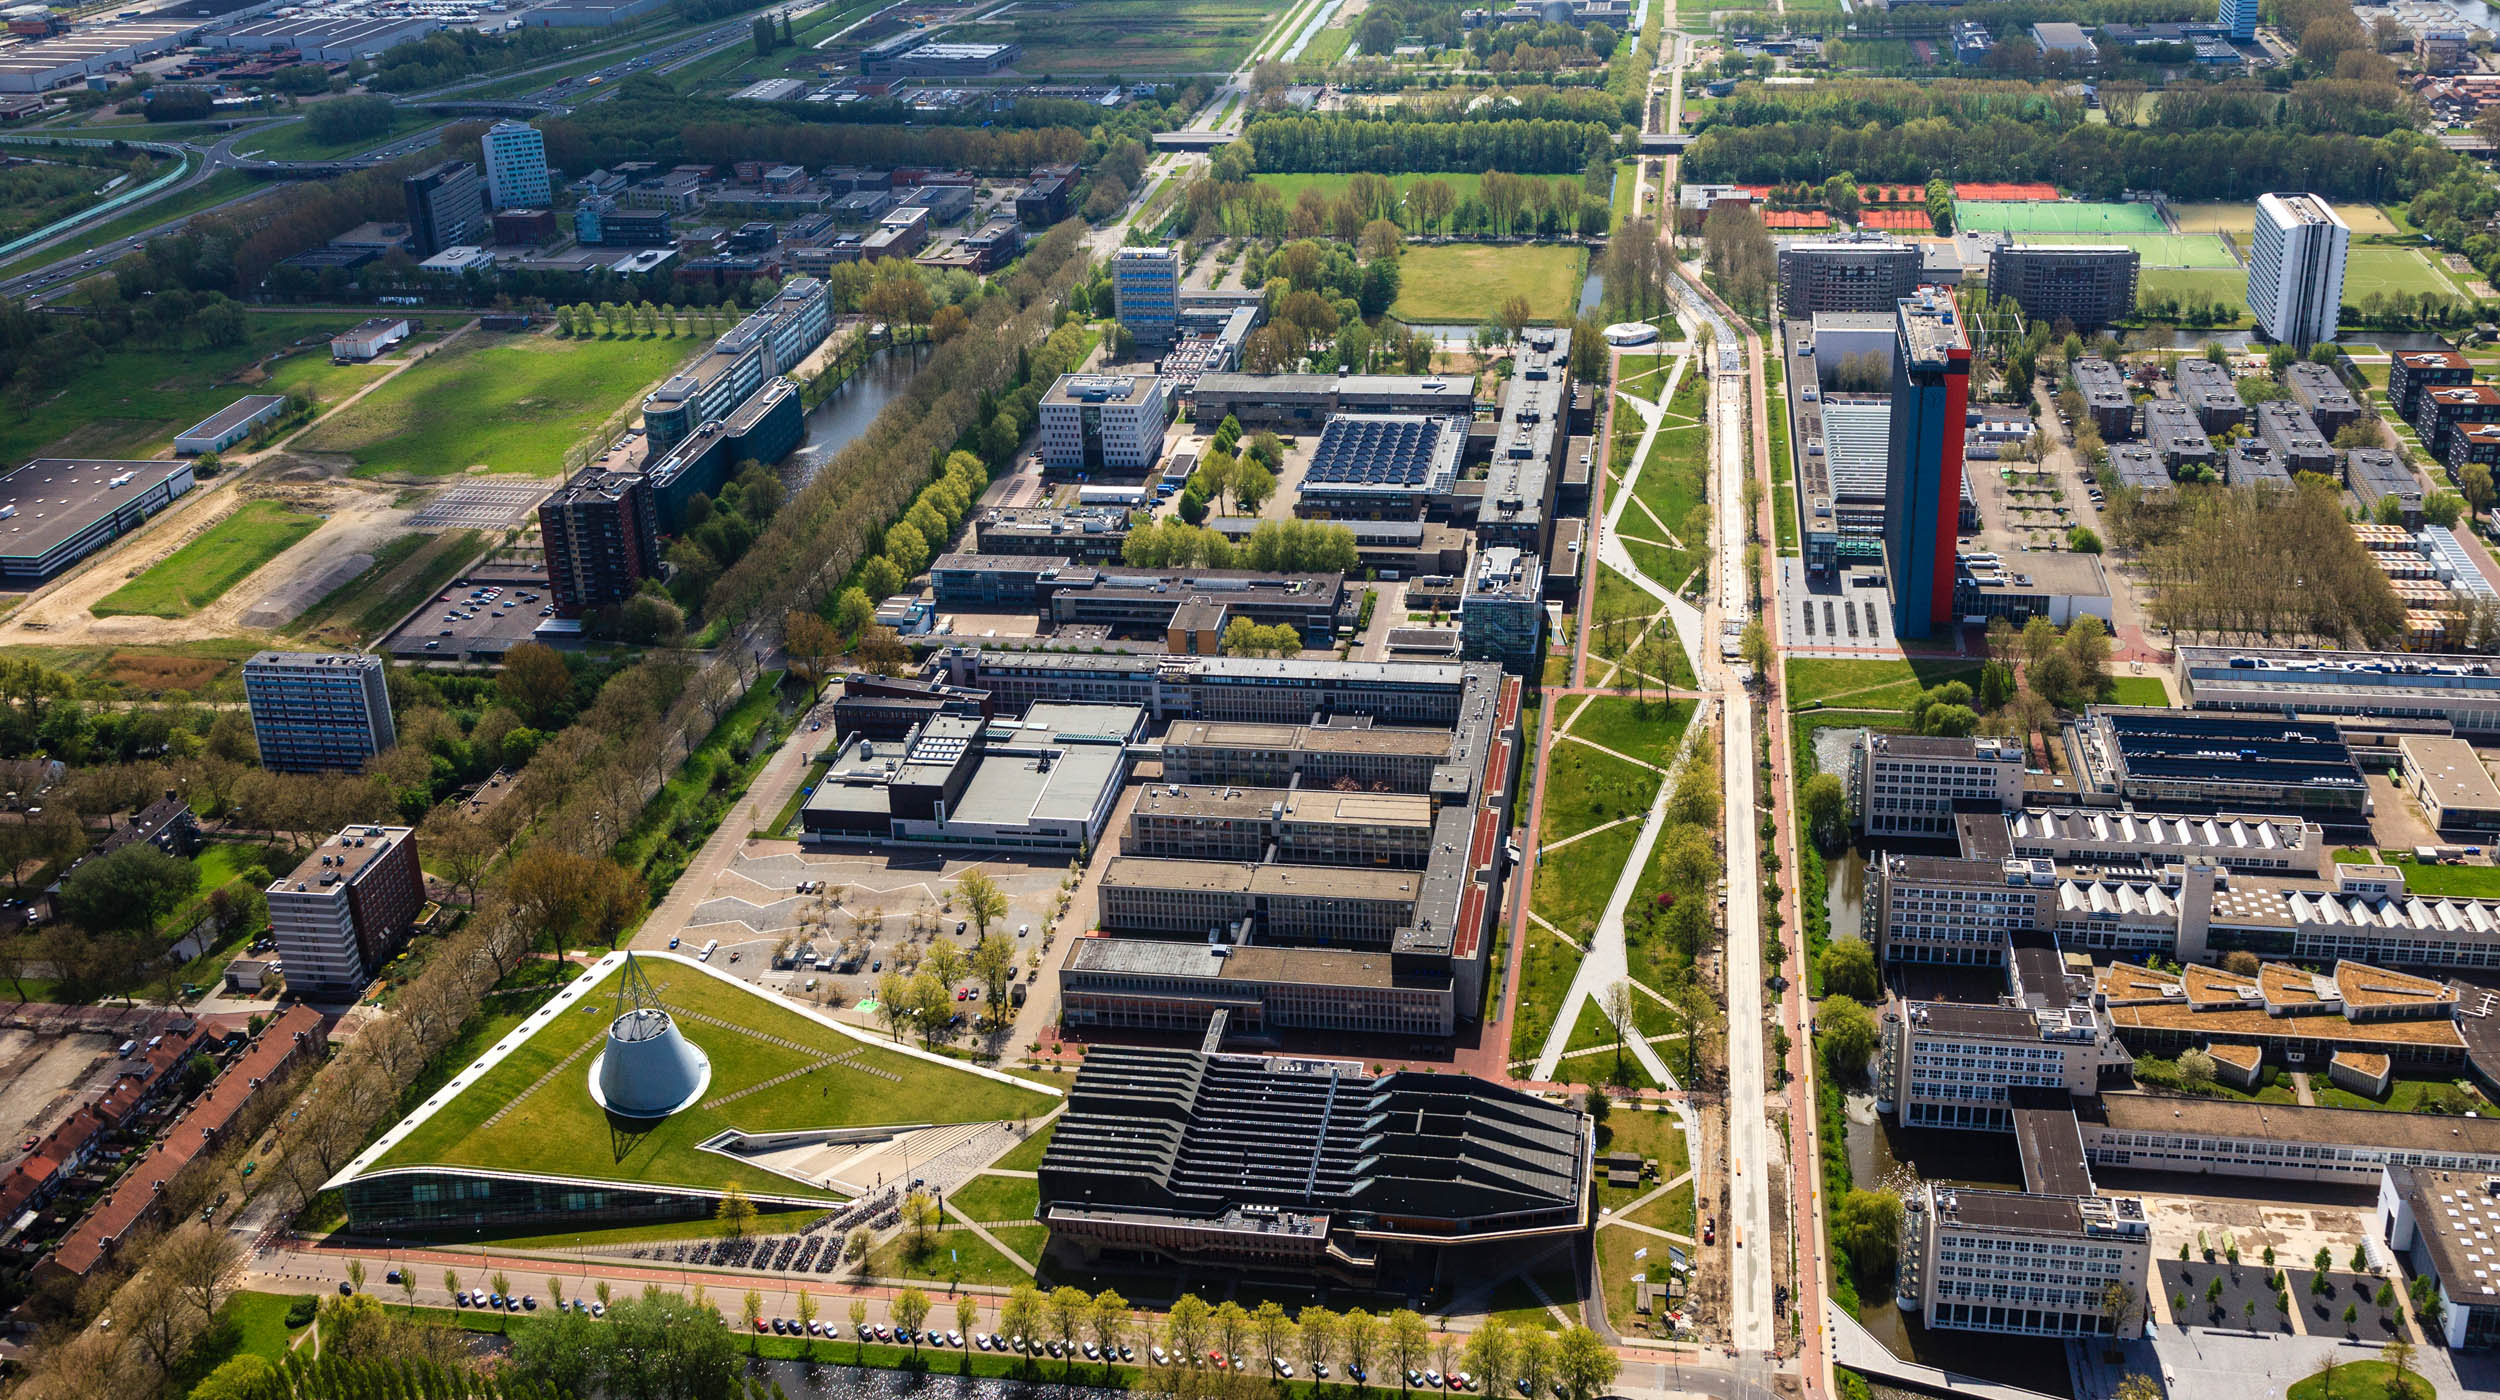
\includegraphics[width=1\textwidth]{images/aerial.jpg}
    \end{figure}
\end{frame}

\begin{frame}
    \delft
    \begin{figure}
        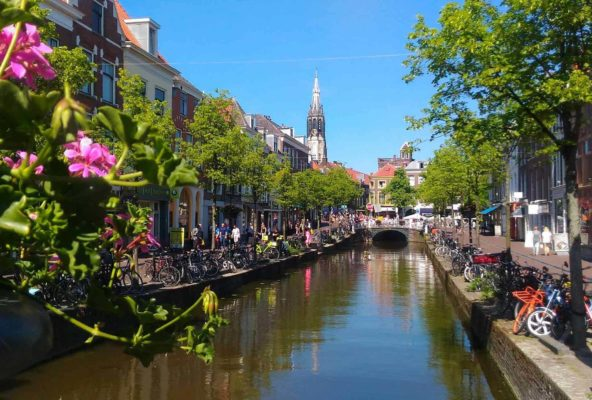
\includegraphics[width=0.9\textwidth]{images/beekje.jpg}
    \end{figure}
\end{frame}

\begin{frame}
    \delft
    \begin{figure}
        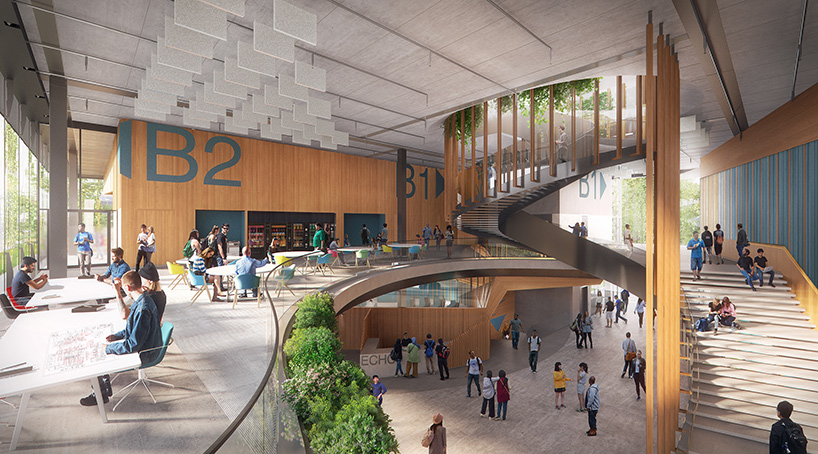
\includegraphics[width=0.9\textwidth]{images/echo.jpg}
    \end{figure}
\end{frame}

\begin{frame}
    \delft
    \begin{figure}
        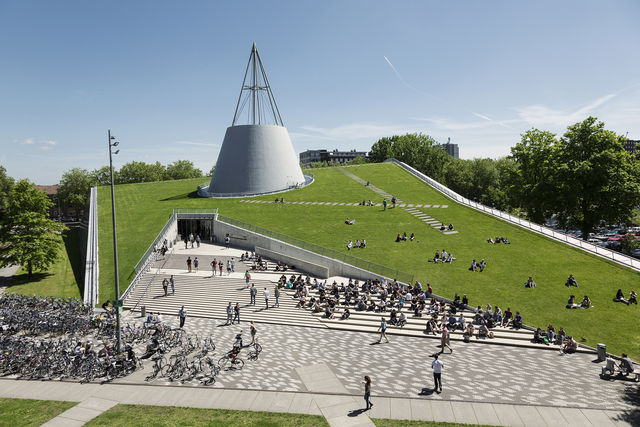
\includegraphics[width=0.9\textwidth]{images/library.jpg}
    \end{figure}
\end{frame}

\begin{frame}
    \delft
    \begin{figure}
        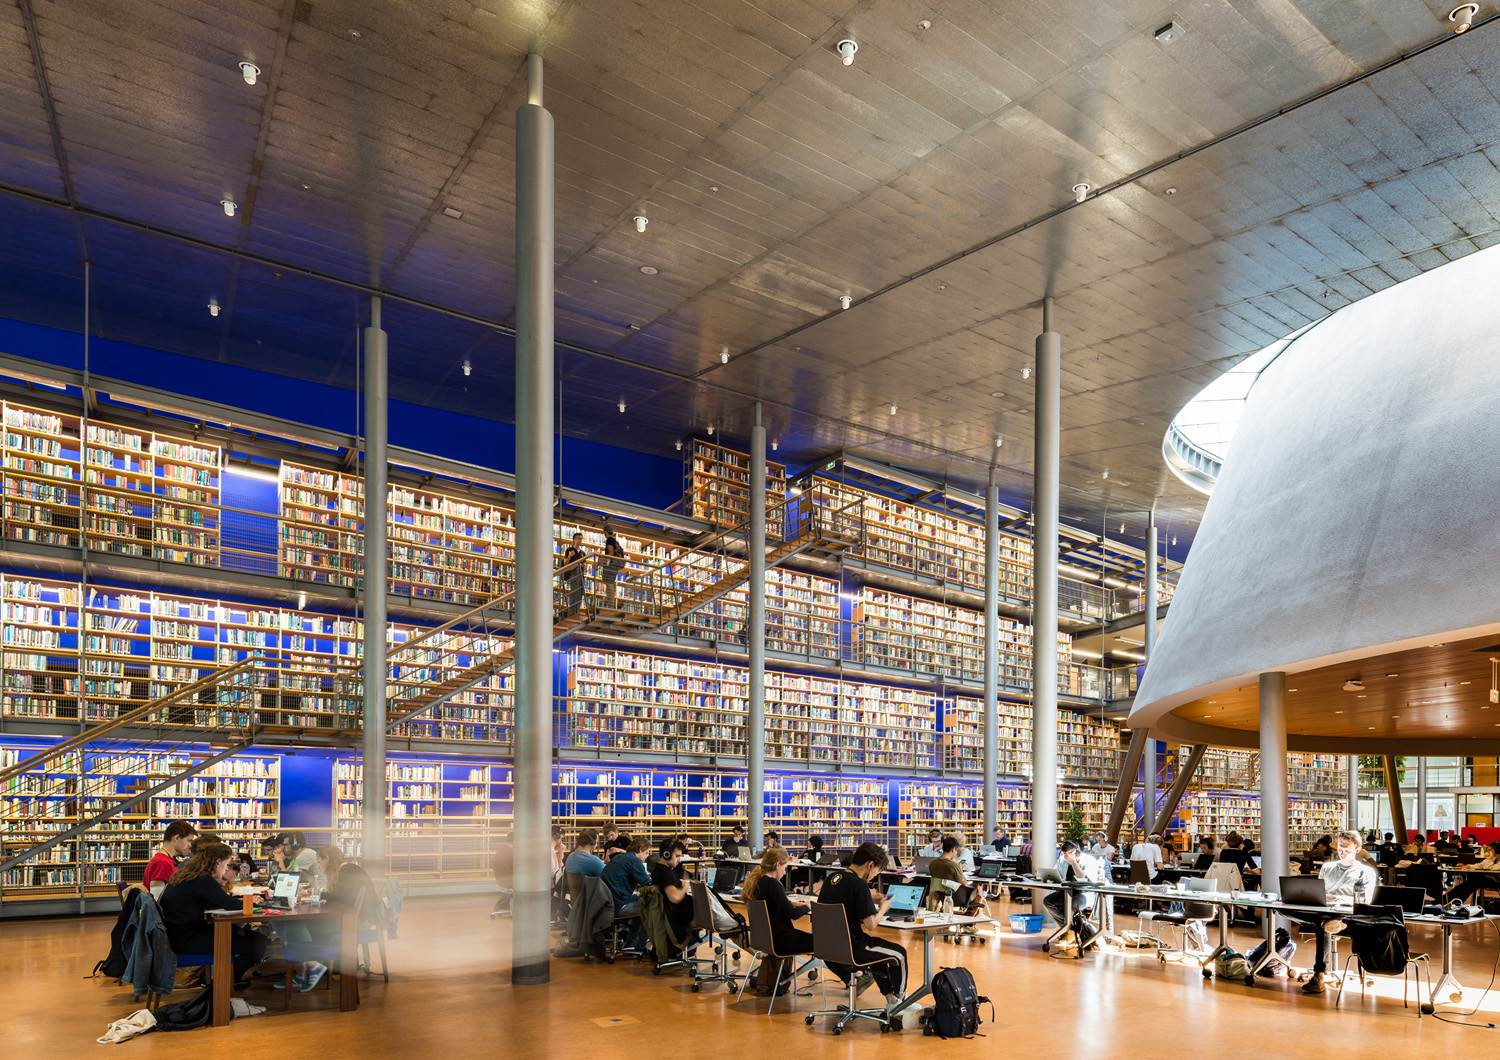
\includegraphics[width=0.9\textwidth]{images/books.jpg}
    \end{figure}
\end{frame}

\begin{frame}
    \delft
    \begin{figure}
        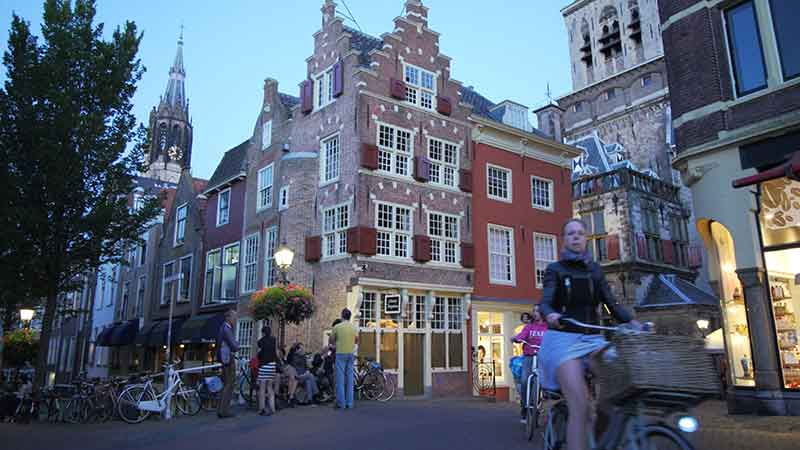
\includegraphics[width=0.9\textwidth]{images/delft-city.jpg}
    \end{figure}
\end{frame}

\begin{frame}
    \delft
    \begin{figure}
        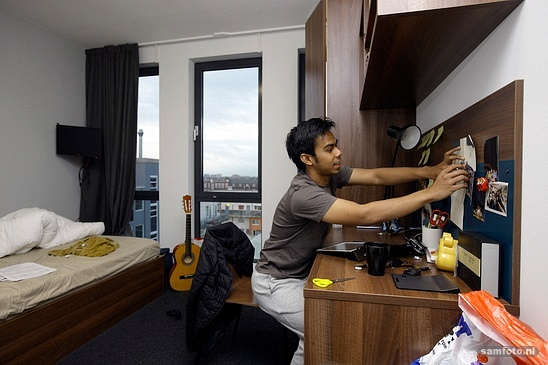
\includegraphics[width=0.9\textwidth]{images/duwo.jpg}
    \end{figure}
\end{frame}

\begin{frame}
    \delft
    \begin{figure}
        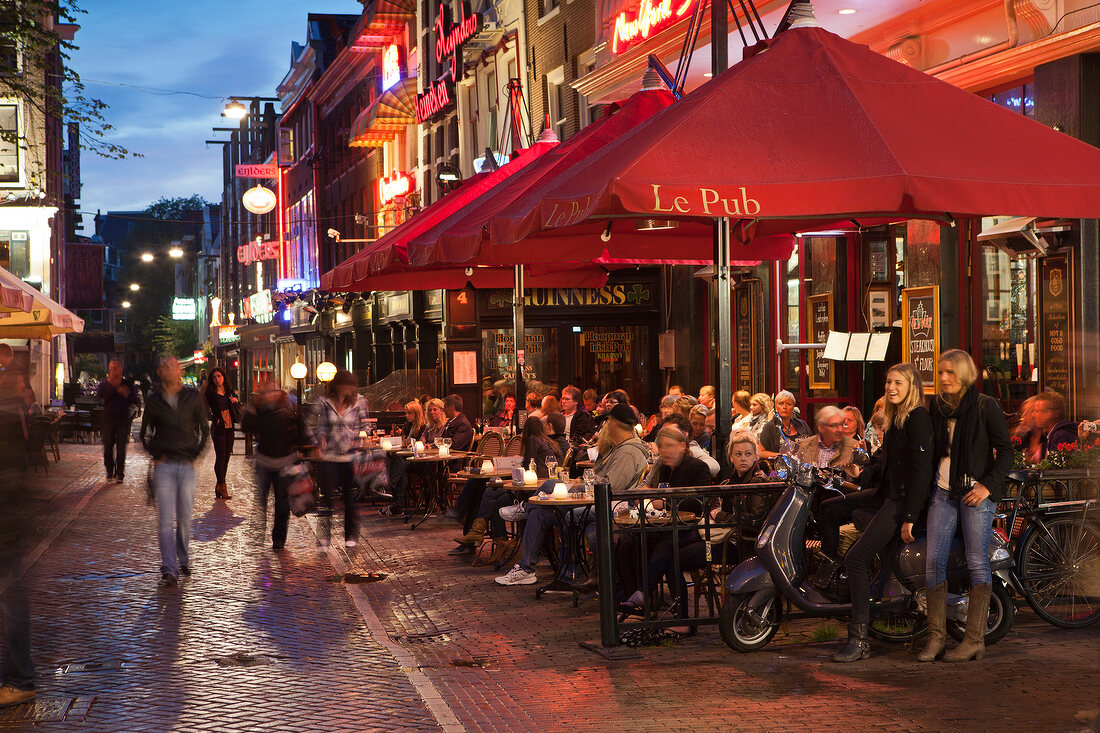
\includegraphics[width=0.9\textwidth]{images/lepub.jpg}
    \end{figure}
\end{frame}

\begin{frame}
    \delft
    \begin{figure}
        \centering
        \begin{tikzpicture}
            \node at (0,0) {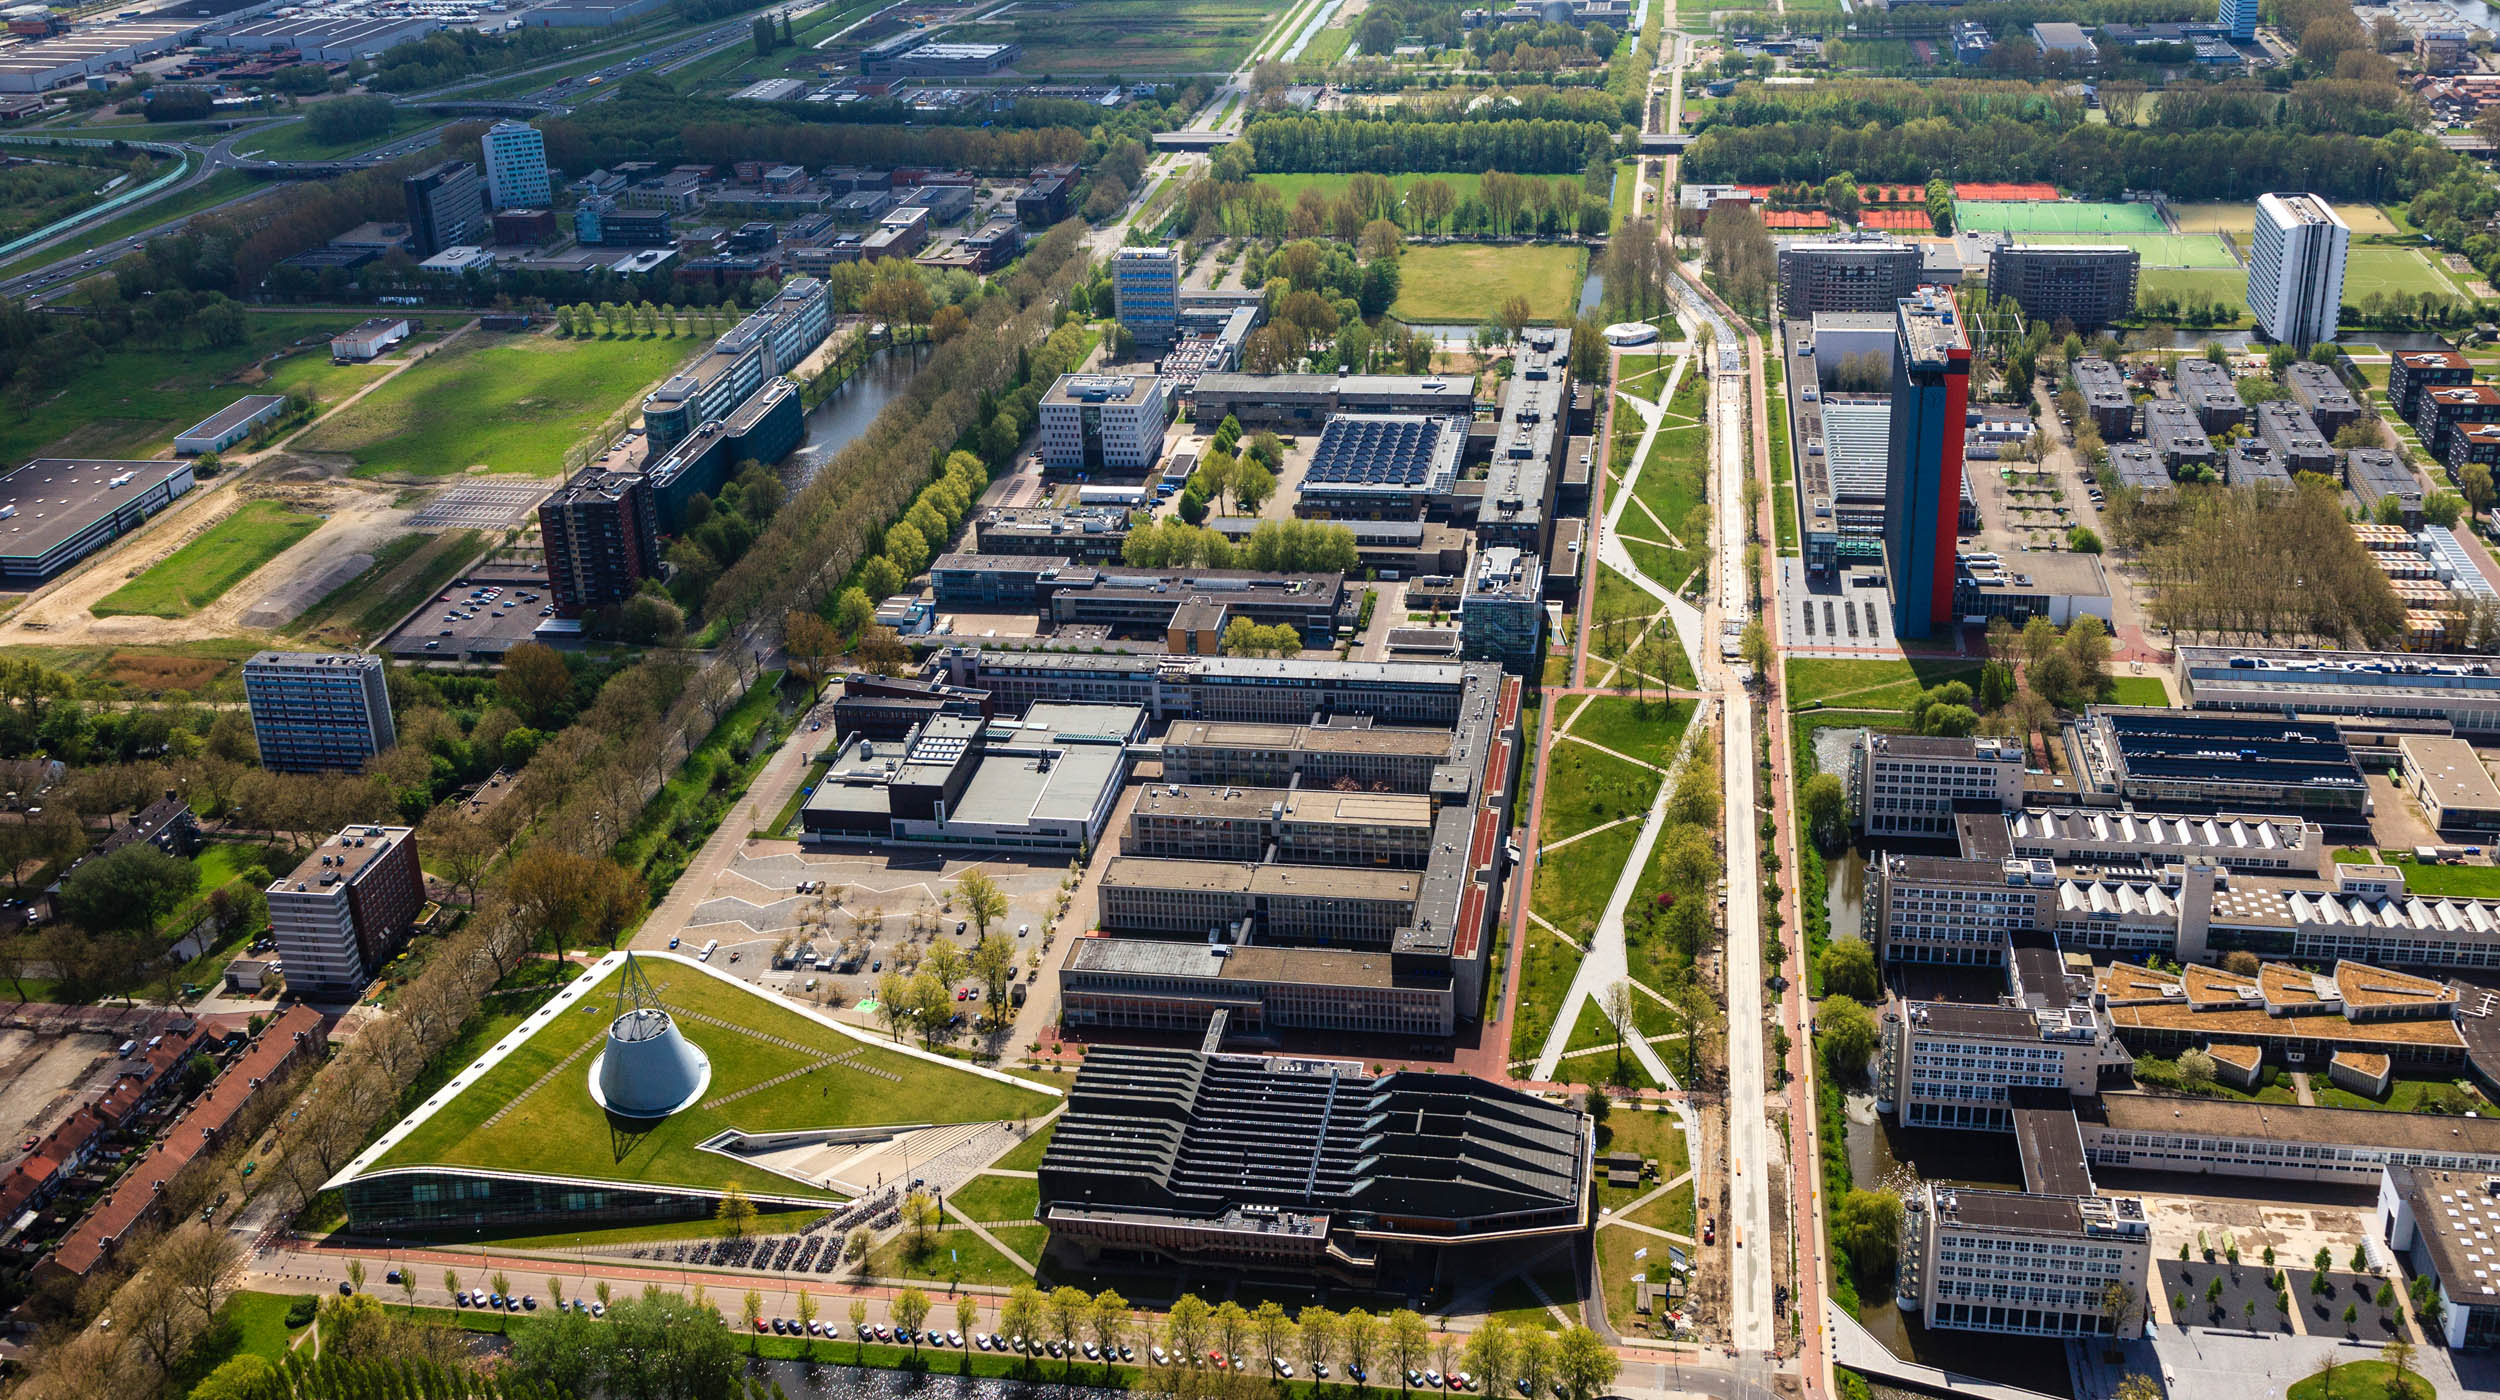
\includegraphics[width=0.9\textwidth]{images/aerial.jpg}};
            \node at (-3.7,-1.5) {
\includegraphics[width=0.3\textwidth]{images/qrcode.png }};
        \end{tikzpicture}
        \small https://www.tudelft.nl/onderwijs/toelating-en-aanmelding/exchange-students
    \end{figure}
\end{frame}





\begin{frame}
\frametitle{Contents}
\tableofcontents
\end{frame}

\section{Part 1}

The four color theorem was initially formulated from a problem in coloring world maps. A map consists of regions that can border other regions on a flat surface. When we talk about a \textit{coloring} of a map, we mean a way to color its regions such that any two neighbors are colored differently.

The actual shape of the regions in our map is not of importance here. The key information that is needed from a map, is the connectivity between regions. Such information can be represented in a \textit{graph} where vertices (circles) correspond to regions. An edge between two vertices then indicates that the two corresponding regions are neighbors.

\begin{figure}[!h]
    \centering
    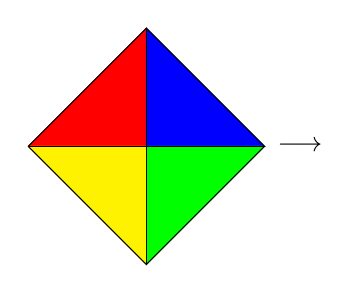
\begin{tikzpicture}[scale=1.5]
        \coordinate (v1) at (-1, 0);
        \coordinate (v2) at (0, 1);
        \coordinate (v3) at (1, 0);
        \coordinate (v4) at (0, -1);
        \coordinate (c) at (0, 0);

        \draw [fill, red] (v1) -- (v2) -- (c) -- (v1);
        \draw [fill, blue] (v2) -- (v3) -- (c) -- (v2);
        \draw [fill, green] (v3) -- (v4) -- (c) -- (v3);
        \draw [fill, yellow] (v4) -- (v1) -- (c) -- (v4);
        \draw (v1) -- (v2) -- (v3) -- (v4) -- (v1);
        \draw (c) -- (v1);
        \draw (c) -- (v2);
        \draw (c) -- (v3);
        \draw (c) -- (v4);
        \node at (1.3, 0) { $\longrightarrow$ };
    \end{tikzpicture} 
    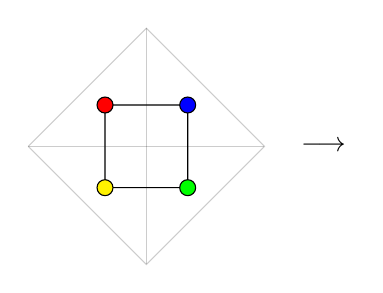
\begin{tikzpicture}[scale=1.5]
        \coordinate (v1) at (-1, 0);
        \coordinate (v2) at (0, 1);
        \coordinate (v3) at (1, 0);
        \coordinate (v4) at (0, -1);
        \coordinate (c) at (0, 0);

        \node[circle, fill, scale=0.01cm, red, draw=black] (m1) at (-0.35, 0.35) { $v_1$ };
        \node[circle, fill, scale=0.01cm, blue, draw=black] (m2) at (0.35, 0.35) { $v_2$ };
        \node[circle, fill, scale=0.01cm, green, draw=black] (m3) at (0.35, -0.35) { $v_3$ };
        \node[circle, fill, scale=0.01cm, yellow, draw=black] (m4) at (-0.35, -0.35) { $v_4$ };

        \draw (m1) -- (m2) -- (m3) -- (m4) -- (m1);
        \draw[opacity=0.2] (v1) -- (v2) -- (v3) -- (v4) -- (v1);
        \draw[opacity=0.2] (c) -- (v1);
        \draw[opacity=0.2] (c) -- (v2);
        \draw[opacity=0.2] (c) -- (v3);
        \draw[opacity=0.2] (c) -- (v4);
        \node at (1.5, 0) { $\longrightarrow$ };
    \end{tikzpicture}  
    \begin{tikzpicture}[scale=1.5, mid arrow/.style={
        postaction={ decorate, decoration={ markings, mark=at position 0.6 with { \arrow[black]{>>} } } } }]
        \coordinate (v1) at (-1, 0);
        \coordinate (v2) at (0, 1);
        \coordinate (v3) at (1, 0);
        \coordinate (v4) at (0, -1);
        \coordinate (c) at (0, 0);

        \node[circle, fill, scale=0.015cm, label=above left:$a$] (m1) at (-0.35, 0.35) { };
        \node[circle, fill, scale=0.015cm, label=above right:$b$] (m2) at (0.35, 0.35) { };
        \node[circle, fill, scale=0.015cm, label=below right:$c$] (m3) at (0.35, -0.35) { };
        \node[circle, fill, scale=0.015cm, label=below left:$d$] (m4) at (-0.35, -0.35) { };

        \draw[mid arrow] (m1) -- (m2);
        \draw (m2) -- (m3) -- (m4) -- (m1);
        \draw[opacity=0.0] (v1) -- (v2) -- (v3) -- (v4) -- (v1);
    \end{tikzpicture}      
    \caption{The translation of a map coloring to a graph coloring. In the last step we replace colors by the letters $a$,$b$,$c$ and $d$ for convenience. We obtain the coloring called $abcd$. graphs. }
    \label{fig:colortut}
\end{figure}

From now on, we will leave the notion of maps and regions behind us and work solely with graphs. When we speak of a coloring, we will generally be working with letters like $abcd$ to indicate the colors on the ring. The order of these colors is indicated by the $\gg$ edge, which is the first edge between the first two vertices. We will also consider two such colorings to be \textit{equal} if they differ only by a renaming of colors.

\begin{definition}
    \label{def:coleq}
    Two colorings $x$ and $y$ are \emph{equal} if they differ only by a renaming of the colors $a,b,c$ and $d$. I.e $abab = acac$.
\end{definition}

\begin{theorem}
    Every planar graph can be colored in at most four colors.
\end{theorem}

With \textit{planar graph} we mean a graph derived from a map as in the first two graphs on the left of Figure \ref{fig:colortut}. Edges are not allowed to cross each other. The proof of this theorem required over a 100 years to complete, despite its simple statement. What would you do to prove such a statement? A first step to the proof is to work with an easier problem instead. This is the five color theorem.
We have seen in the proof of the five color theorem that a vertex surrounded by five or less neighbors can always be colored using one of five colors, even if all of its neighbors initially use all five colors. If we have only four colors available, we will find that it is no longer guaranteed that we can free a color. This is what Alfred Kempe tried to do when he gave the first false proof of the four color theorem.

If we look at the key idea, we see that if one half of a graph is isolated from another half by a group of boundary vertices, we can color this isolated part regardless of the colors on the boundary. Naturally, the fundamental shape that seperates a graph in two halves is a \textit{ring}.

\begin{definition}
    A \emph{ring} of $n$ vertices $R_n$ in a planar graph $G$ is an induced cycle of $G$.
\end{definition}

\begin{figure}[!ht]
    \centering
    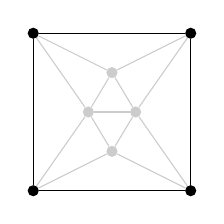
\begin{tikzpicture}
        \node[circle, fill, scale=0.015cm] (l1) at (-1, -1) { };
            \node[circle, fill, scale=0.015cm] (l2) at (-1, 1) { };
            \node[circle, fill, scale=0.015cm] (l3) at (1, 1) {};
            \node[circle, fill, scale=0.015cm] (l4) at (1, -1) {};
            \node[circle, fill, scale=0.015cm, opacity=0.2] (m1) at (0, 0.5) {};
            \node[circle, fill, scale=0.015cm, opacity=0.2] (m2) at (-0.3, 0) {};
            \node[circle, fill, scale=0.015cm, opacity=0.2] (m3) at (0.3, 0) {};
            \node[circle, fill, scale=0.015cm, opacity=0.2] (m4) at (0, -0.5) {};

            \draw (l1) -- (l2) -- (l3) -- (l4) -- (l1);
            \draw[opacity=0.2] (m1) -- (m2) -- (m4) -- (m3) -- (m1);
            \draw[opacity=0.2] (m2) -- (m3);
            \draw[opacity=0.2] (m1) -- (l2);
            \draw[opacity=0.2] (m1) -- (l3);
            \draw[opacity=0.2] (m2) -- (l1);
            \draw[opacity=0.2] (m2) -- (l2);
            \draw[opacity=0.2] (m3) -- (l3);
            \draw[opacity=0.2] (m3) -- (l4);
            \draw[opacity=0.2] (m4) -- (l1);
            \draw[opacity=0.2] (m4) -- (l4);
    \end{tikzpicture}
    \hspace{1cm}
    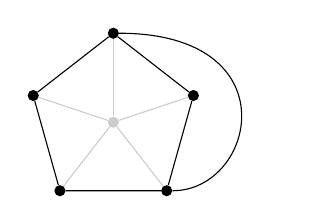
\begin{tikzpicture}[scale=1.13]
        \node[circle, fill, scale=0.015cm, opacity=0.2] (c) at (0, 0) {};


        \node[circle, fill, scale=0.015cm] (l1) at (0, 1) { };
        \node[circle, fill, scale=0.015cm] (l2) at (0.9, 0.30) { };
        \node[circle, fill, scale=0.015cm] (l3) at (0.6, -0.77) {};
        \node[circle, fill, scale=0.015cm] (l4) at (-0.6, -0.77) {};
        \node[circle, fill, scale=0.015cm] (l5) at (-0.9, 0.30) {};

        \draw[opacity=0.2] (c) -- (l1);
        \draw[opacity=0.2] (c) -- (l2);
        \draw[opacity=0.2] (c) -- (l3);
        \draw[opacity=0.2] (c) -- (l4);
        \draw[opacity=0.2] (c) -- (l5);
        \draw (l1) -- (l2) -- (l3) -- (l4) -- (l5) -- (l1);
        \draw (l1) .. controls +(2,0) and +(1,0) .. (l3);
    \end{tikzpicture}
    \caption{An example of the ring $R_4$ surrounding a graph on four vertices (left). An example of an invalid ring $R_5$ (right). }
    \label{fig:ring}
\end{figure}

The vertex of ring $R_1$ can not have a single edge to itself, instead, it acts as a bridge from one part of a graph to the other. For rings present in graphs, we are interested in which colorings are possible on them, called \textit{ring colorings}. The set of these colorings for a graph $G$ we shall define. It turns out that the rings $n\geq 4$ are already reducible configurations. Therefore, all future configurations will only contain triangles (the ring $R_3$), they will be \textit{triangulations}.


\begin{definition}
    The set of all \emph{valid} 4-colorings of a ring $R$ in a planar graph $G$ is given by $\Phi(R \subset G)$ or $\Phi(G)$ if $R$ is clear from the context. 
\end{definition}
\begin{definition}
    The set of all valid ring colorings of $R_n$ is given by $\Phi(n) = \Phi(R_n)$.
\end{definition}

\begin{theorem}
    \label{thm:ringsarered}
    The ring $R_n$ with $n\geq 4$ is reducible in every planar graph $G$.
\end{theorem}

\begin{proof}
Let $R_n$ be contained in $G$. Since the interior of $R_n$ is empty and $n\geq4$, we may contract the two non-neighboring ring vertices $v_1, v_3$ to a new vertex $u$. As a result, we obtain the graph $G'$ on one less vertex. See Figure \ref{fig:ringcontract}.

Given a 4-coloring of $G'$. Because $R_n$ is a ring, there will be no edges between the ring vertices $v_1$ and $v_3$. Therefore, we may give $v_1$ and $v_3$ the same color as $u$ without issue. Let the other vertices of $G$ be given the same color as their $G'$ counterparts. Then we have obtained a 4-coloring of $G$.

\end{proof}

\needspace{4cm}
\begin{figure}[!h]
    \centering
    \begin{tikzpicture}[scale=0.7]
        \node (l1) at (-1, -1) { $a$ };
        \node (l2) at (-1, 1) { $b$ };
        \node (l3) at (1, 1) { $c$ };
        \node (l4) at (1, -1) { $b$ };

        \draw (l1) -- (l2) -- (l3) -- (l4) -- (l1);
        \node (impl) at (2.3, 0) { $\Longleftrightarrow$ };
        \draw[dotted, thick] (l2) -- (l4);
    \end{tikzpicture}
    \begin{tikzpicture}[scale=0.7]
        \node (l1) at (-1, -1) { $a$ };
        \node[opacity=0.2] (l2) at (-1, 1) { $b$ };
        \node (l3) at (1, 1) { $c$ };
        \node[opacity=0.2] (l4) at (1, -1) { $b$ };
        \node (c) at (0, 0) { $b$ };

        \draw (l1) -- (c) -- (l3);
        \draw[dotted, thick, opacity=0.2] (l2) -- (c) -- (l4);
    \end{tikzpicture}
    \caption{The ring $R_4$ being contracted to a smaller graph $G'$. The coloring of $G'$ can be reversed to a coloring of $G$.}
    \label{fig:ringcontract}
\end{figure}
\begin{frame}
    
\includegraphics[width=\textwidth]{images/break1.png}
    We will be back in 5 minutes.
\end{frame}

\section{Part 2}
\subsection{0-reducibility of ring $R_4$}

\begin{frame}
    \frametitle{0-reducibility of ring $R_4$}

    \begin{theorem}<1->
        The ring $R_4$ is 0-reducible
    \end{theorem}
    \uncover<2->{
        \textit{Proof.} We will show that there is a common ring coloring for any $M+R_4$ and $\confg$. Let the ring colorings of the two graphs be given by
        \begin{equation}
            \I = \Phi(M+R_4) \quad \text{and} \quad \II = \Phi(\confg).
        \end{equation}
    }
    \uncover<3->{
        The situation is sketched below.
        \begin{figure}[!ht]
        \centering
        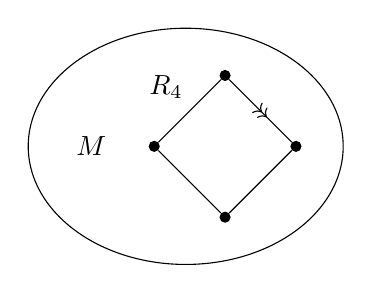
\begin{tikzpicture}[mid arrow/.style={
            postaction={ decorate, decoration={ markings, mark=at position 0.6 with { \arrow[black]{>>} } } } }]
            \draw[fill=white] (-0.5, 0) ellipse (2cm and 1.5cm);
            \node (m) at (-1.7, 0) {$M$};
            \node at (-0.75, 0.75) {$R_4$};
    
            \node[circle, fill, scale=0.015cm] (l1) at (0, 0.9) { };
            \node[circle, fill, scale=0.015cm] (l2) at (0.9, 0) { };
            \node[circle, fill, scale=0.015cm] (l3) at (0, -0.9) {};
            \node[circle, fill, scale=0.015cm] (l4) at (-0.9, 0) {};
    
            \draw[mid arrow] (l1) -- (l2);
            \draw (l2) -- (l3) -- (l4) -- (l1);
        \end{tikzpicture}
        \begin{tikzpicture}[mid arrow/.style={
            postaction={ decorate, decoration={ markings, mark=at position 0.6 with { \arrow[black]{>>} } } } }]
            \draw[opacity=0] (-0.5, 0) ellipse (2cm and 1.5cm);
            \node at (-0.75, 0.75) {$R_4$};
            \node[inner sep=1mm] (c) at (0, 0) {$\core$};
    
            \node[circle, fill, scale=0.015cm] (l1) at (0, 0.9) { };
            \node[circle, fill, scale=0.015cm] (l2) at (0.9, 0) { };
            \node[circle, fill, scale=0.015cm] (l3) at (0, -0.9) {};
            \node[circle, fill, scale=0.015cm] (l4) at (-0.9, 0) {};
    
            \draw[mid arrow] (l1) -- (l2);
            \draw (l2) -- (l3) -- (l4) -- (l1);
            \draw[opacity=0.2] (l1) -- (c);
            \draw[opacity=0.2] (l2) -- (c); 
            \draw[opacity=0.2] (l3) -- (c);
            \draw[opacity=0.2] (l4) -- (c);
        \end{tikzpicture}
    \end{figure}}
\end{frame}

\begin{frame}
    \frametitle{0-reducibility of ring $R_4$}

    \uncover<1->{Both parts have a plain ring $R_4$, which we have shown to be reducible. Therefore, we may contract any two opposing vertices.}
    
    \uncover<2->{This gives us a guarantee on two colorings in both sets I and II.

    \begin{equation}
        \left\{\begin{matrix}
            abab \;\;\text{or}\;\; abac, \\
            baba \;\;\text{or}\;\; baca
        \end{matrix}\right\} \subset I,II.
    \end{equation}}

    \uncover<3->{
        Therefore, we have 4 possible options for guaranteed colorings in I and II, 3 of which are unique.

        \begin{equation}
            \circled{1} = \{ abab \}, \quad \circled{2} = \left\{ \begin{matrix}abab \\ baca\end{matrix} \right\}, \quad \circled{3} = \left\{ \begin{matrix}abac \\ baca \end{matrix} \right\}.
        \end{equation}
    }
\end{frame}

\begin{frame}
    \frametitle{0-reducibility of ring $R_4$}
    \begin{equation*}
        \circled{1} = \{ abab \}, \quad \circled{2} = \left\{ \begin{matrix}abab \\ baca\end{matrix} \right\}, \quad \circled{3} = \left\{ \begin{matrix}abac \\ baca \end{matrix} \right\}.
    \end{equation*}

    \uncover<1->{We consider the 3 pairs that can occur for I and II. Two pairs already have a common coloring from the start.}
    
    \uncover<2->{The only pair that does not directly have a common coloring is $\circled{1}$ and $\circled{3}$. }
\end{frame}

\begin{frame}
    \frametitle{0-reducibility of ring $R_4$}
    
    \uncover<1->{Let $\{ abab \} \subset \I$ and $\{ abac, baca \} \subset \II$ be guaranteed colorings. }
    
    \uncover<2->{Suppose that in the coloring $\I(abab)$ we have $\chain{v_1}{v_3}{ad}$.

    \begin{equation}
        \begin{aligned}
            \I(abab) &= \scheme{a,b,a,b}{13d} \compat \II(abac) \\
            \I(abab) &= \scheme{a,b,a,b}{13d-} \compat \I(abcb) = \II(baca).
        \end{aligned}
    \end{equation}    
    
    Therefore, the guaranteed colorings always lead to a common coloring $\qedsymbol$.
    }
    
\end{frame}

\begin{frame}
    \frametitle{Examples of reducible configurations on $R_4$}
    \centering
    \begin{figure}
        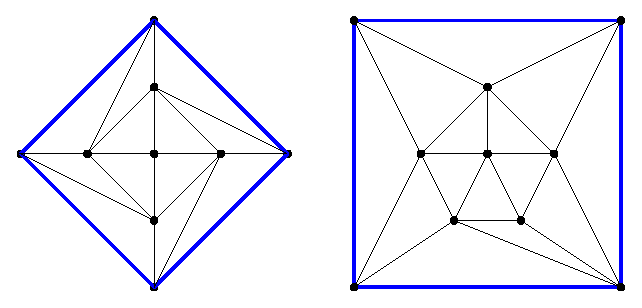
\includegraphics[width=0.7\textwidth]{images/example4.eps}
    \end{figure}

    Because $R_4$ is 0-reducible, the interior of \textbf{any} configuration on $R_4$ can be removed.
\end{frame}
\subsection{Reducibility of configurations on $R_5$}

Recall that every planar graph has a vertex with $\deg(v) \leq 5$. If we add edges between the neighbors of this vertex, then we obtain the rings $R_1$ thru $R_5$. We have seen the 0-reducibility of configurations on the first four. Therefore, if we could prove that every configuration on $R_5$ is 0-reducible, any planar graph would be reducible and the four color theorem would follow. Many people have tried to show this and failed, so let this serve as an warning as to why we should prove 1-reducibility instead.

\begin{theorem}
    A configuration $\confg$ on $R_5$ is 1-reducible in all planar graphs $M$ if it has a 3-coloring, or all planar graphs with $|M|>1$ if it does not.
\end{theorem}

\begin{proof}
We may consider a configuration with $|\confg| > 1$. Let the planar graph $M$ be arbitary. We will again use the convention of the sets $\I$ and $\II$ for the ring colorings.

\begin{equation}
    \I = \Phi(M+S) \quad \text{and} \quad \II = \Phi(\confg).
\end{equation}

The heart of this proof depends on a guaranteed 3-coloring in both $\I$ and $\II$. Because we may set our reducer $S=W_5$ (See Figure \ref{fig:reducertut}), we are guaranteed of the following colorings.
\begin{equation}
    \Phi^\star(5) \;\subset\; \I, \II \quad\text{and}\quad \Phi^{W_5} \subset \I,\II.
\end{equation}

To justify that $\Phi^{W_5} \subset \II$ in case a 3-coloring is not given by $\confg$ from the start, let us add a single vertex $v$ to the configuration $\confg$ as illustrated in Figure \ref{fig:confg3col}. This results in the graph $\confg'$ on 1 more vertex. We may assume that $\confg'$ has a 4-coloring because $\confg' < M+\confg$ from our assumption that $|M| > 1$. In particular, $\confg'$ will have a 3-coloring on the ring from $W_5$. We may remove $v$ in this 3-coloring to obtain a 3-coloring of $\confg$. Therefore $\Phi^{W_5} \subset \Phi(\confg)$. 

\needspace{5cm}
\begin{figure}
    \centering
    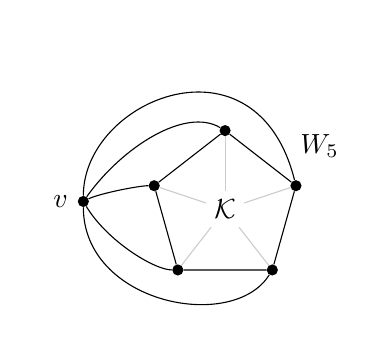
\begin{tikzpicture}
        \draw[opacity=0] (-0.5, 0) ellipse (2cm and 1.5cm);
        \node[fill=white] at (1.2, 0.8) {$W_5$};
        \node[inner sep=1mm] (c) at (0, 0) {$\core$};
        \node[circle, fill, scale=0.015cm] (l1) at (0, 1) { };
        \node[circle, fill, scale=0.015cm] (l2) at (0.9, 0.30) { };
        \node[circle, fill, scale=0.015cm] (l3) at (0.6, -0.77) {};
        \node[circle, fill, scale=0.015cm] (l4) at (-0.6, -0.77) {};
        \node[circle, fill, scale=0.015cm] (l5) at (-0.9, 0.30) {};
        \node[circle, fill, scale=0.015cm, label=left:$v$] (e) at (-1.8, 0.1) { };

        \draw (e) .. controls +(0.2, 0.1) and + (-0.2, 0.0) .. (l5);
        \draw (e) .. controls +(0.3, -0.5) and +(-0.3,0) .. (l4);
        \draw (e) .. controls +(0.0,-1.3) and +(-0.5,-0.8) .. (l3);
        \draw (e) .. controls +(0.0,+1.3) and +(-0.5,+2) .. (l2);
        \draw (e) .. controls +(0.5,0.7) and +(-0.5, 0.3) .. (l1);

        \draw[opacity=0.2] (c) -- (l1);
        \draw[opacity=0.2] (c) -- (l2);
        \draw[opacity=0.2] (c) -- (l3);
        \draw[opacity=0.2] (c) -- (l4);
        \draw[opacity=0.2] (c) -- (l5);
        \draw (l1) -- (l2) -- (l3) -- (l4) -- (l5) -- (l1);
    \end{tikzpicture}  
    \caption{The modified configuration $\confg'$ used to guarantee a 3-coloring of $\confg$.}
    \label{fig:confg3col}
\end{figure}


A special property of 3-colorings on $R_5$ is that there will always be a single vertex colored uniquely, we call this the \textit{marked vertex}. This vertex acts as a kind of 'pivot' to tell if two 3-colorings are \textit{adjacent}. These two concepts are key to the proof.

\begin{definition}
    The uniquely-colored vertex of a 3-coloring of $R_5$ is called the \emph{marked vertex}, indicated by an underline such as in $\underline{c}abab$.
\end{definition}
\begin{definition}
    Two 3-colorings of $R_5$ are called \emph{adjacent} if they have adjacent marked vertices, such as in $\underline{c}abab$ and $a\underline{c}bab$.
\end{definition}

Since we have guaranteed 3-colorings for both $\I$ and $\II$, we can split up our proof into 3 cases.

\begin{enumerate}
    \item $\I$ and $\II$ have an adjacent coloring ($\underline{c}abab$ and $a\underline{c}bab$).
    \item $\I$ and $\II$ have a non-adjacent coloring ($\underline{c}abab$ and $ab\underline{c}ab$).
    \item $\I$ and $\II$ have a coloring with the same marked vertex ($\underline{c}abab$ and $\underline{d}cbcb$). These are already equal, so we are done.
\end{enumerate}

Therefore, we only need to consider the cases \circled{1} and \circled{2}. We will prove two lemma's to this end. Their relation is illustrated below.

\begin{equation*}
    \begin{aligned}
    \circled{2} \implies\; &\circled{1}\quad \text{or} \quad \text{common coloring} \quad\quad \text{(Lemma \ref{lem:r5_first})} \\
    &\downarrow \\
    &\circled{1} \implies\;\text{common coloring}\quad\quad \text{(Lemma \ref{lem:r5_second})}
    \end{aligned}
\end{equation*}

\begin{lemma}
    \label{lem:r5_first}
    If $\I$ and $\II$ have a non-adjacent coloring, then they either have an adjacent coloring or a common coloring.
\end{lemma}

\begin{proof}
Let two non-adjacent colorings $\I(\underline{c}abab)$ and $\II(ab\underline{c}ab)$ be given. We make a case dinstinction whether the chain $v_3 \stackrel{bc}{\frown} v_5$ exists in $\II(ab\underline{c}ab)$ or not. 

\begin{equation}
    \label{eq:abcab}
    \begin{aligned}
        \II(ab\underline{c}ab) &=\scheme{a,b,c,a,b}{35b} \compat \II(abcdb), \\
        \II(ab\underline{c}ab) &= \scheme{a,b,c,a,b}{35b-} \compat \II(a\underline{c}bab).
    \end{aligned}
\end{equation}

The second case results in a coloring adjacent to $\I(\underline{c}abab)$. For the first case, we consider the coloring $\I({*}b{*}{*}b)$. The two adjacent ${*}$-colors must be different from each other and $b$, therefore we may assume that we have $\I({*}bcdb)$. The last ${*}$-color reveals 3 possibilities.

\begin{equation}
    \begin{matrix*}[l]
        \I(abcdb) \quad\quad =&\II(abcdb) \; \text{from (\ref{eq:abcab}),}  \\
        \I(cbc\underline{d}b) \;\; \text{adjacent to}&\II(ab\underline{c}ab), \;  \\
        \I(db\underline{c}db) \quad\quad =&\II(ab\underline{c}ab).
    \end{matrix*}
\end{equation}

Therefore we obtain either a common coloring or an adjacent coloring. Note that the pair of non-adjacent colorings we chose is the only unique one on $R_5$ (up to rotational symmetry).
\end{proof}

\begin{lemma}
    \label{lem:r5_second}
    If I and II have an adjacent coloring, then they have a common coloring.
\end{lemma}

\begin{proof}

Let two adjacent colorings $\I(\underline{c}abab)$ and $\II(a\underline{c}bab)$ be given. We make a case dinstinction whether the chain $\chain{v_3}{v_5}{bd}$ exists in $\II(a\underline{c}bab)$ or not.

\begin{equation}
    \label{eq:acdab}
    \begin{aligned}
        \II(a\underline{c}bab) &= \scheme{a,c,b,a,b}{35d} \compat \I(\underline{c}abab). \\
        \II(a\underline{c}bab) &= \scheme{a,c,b,a,b}{35d-} \compat \II(acdab).
    \end{aligned}
\end{equation}

The first case leads to a common coloring. For the second case,
we consider the coloring $\I(a{*}{*}a{*})$. We may again assume to have $\I(acda{*})$. Then the 3 remaining possibilities for the ${*}$-color are

\begin{equation*}
    \begin{matrix*}[l]
        \I(acdab) \quad =& \II(acdab), \;\text{from (\ref{eq:acdab})},\\
        \I(ac\underline{d}ac) \quad =\;\; \text{shifted $+2$}& \I(\underline{c}abab), \\
        \I(a\underline{c}dad) \quad =& \II(a\underline{c}bab).
    \end{matrix*}
\end{equation*}

If we do not obtain common colorings, we may repeat this procedure with $\II(a\underline{c}bab)$ and $\I(ac\underline{d}ac)$ to continously shift the marked vertex two to the right. The pattern that arises is illustrated in Figure \ref{table:ringpattern5}.

\begin{figure}[!ht]
    \centering
    \begin{tabular}{c|ccccc:c}
         & $v_1$ & $v_2$  & $v_3$  & $v_4$ & $v_5$ & $v_1$  \\
        \hline
        1 & \I & \II &    &     &    & \I  \\
        2 &    & \II & \I &     &    &     \\
        3 &    &     & \I & \II &    &     \\
        4 &    &     &    & \II & \I &     \\
        5 &    &     &    &     & \I & \II \\
    \end{tabular}
    \caption{Marked vertices of $\I$ and $\II$ obtained by repetition of the earlier procedure.  Every step shifts the leftmost marked vertex two to the right. }
    \label{table:ringpattern5}
\end{figure}

At iteration 5, we obtain that $\II$ has the same marked vertex $v_1$ as $\I$. Therefore, by repetition we obtain that

\begin{equation}
    \II(a\underline{c}bab) \rightarrow \II(aba\underline{c}b) \rightarrow \II(\underline{c}abab) = \I(\underline{c}abab).
\end{equation}

\end{proof}

Therefore, adjacent colorings imply a common coloring for $\I$ and $\II$. Combining these two lemmas yields a guaranteed common ring coloring for $\I$ and $\II$ regardless of the case.

\end{proof}
\begin{frame}
    
\includegraphics[width=\textwidth]{images/break2.jpg}
    We will be back in 5 minutes.
\end{frame}

\section{Part 3}
\section{D-Reducibility}
\label{sec:dreduce}

We have seen that the ring $R_4$ is 0-reducible and the that the ring $R_5$ is 1-reducible. This essentially provides us with an two infinite classes of reducible configurations. However, it is not yet guaranteed that every planar graph contains such a $k$-reducible configuration on $R_4$ or $R_5$. Therefore, we must still look for more reducible configurations.

Naturally, we might try to examine the $k$-reducibility of $R_6$ and beyond. However, as we have seen in the increase in complexity for the 1-reducibility of $R_5$, this is a very tough problem. There are much more cases to consider for the ring $R_6$ than for $R_4$ and $R_5$. However, the difficulty of $k$-reducibility lies in the fact the we try to prove the reducibility of \textit{all} configurations $\confg$ on $R_n$ at once. Individual configurations are much easier to examine. 

Let us introduce the idea of D-reducibility, by working with an example. The very first, smallest and most famous configuration used in the proof of the four color theorem is the \textit{Birkhoff Diamond}  ($\text{Bir}\Diamond$). It is a configuration on $R_6$ with 4 vertices in the core.

\begin{figure}[!ht]
    \centering
    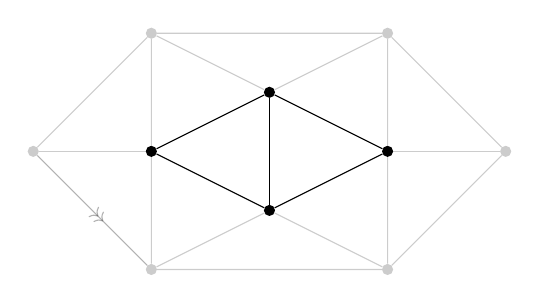
\begin{tikzpicture}[scale=1.5, mid arrow/.style={
        postaction={ decorate, decoration={ markings, mark=at position 0.6 with { \arrow[black]{>>} } } } }]
        \node[circle, fill, scale=0.015cm, opacity=0.2] (l1) at (-2, 0) { };
        \node[circle, fill, scale=0.015cm, opacity=0.2] (l2) at (-1, 1) { };
        \node[circle, fill, scale=0.015cm] (l3) at (-1, 0) {};
        \node[circle, fill, scale=0.015cm, opacity=0.2] (l4) at (-1, -1) {};

        \node[circle, fill, scale=0.015cm, opacity=0.2] (r1) at (2, 0) {};
        \node[circle, fill, scale=0.015cm, opacity=0.2] (r2) at (1, 1) {};
        \node[circle, fill, scale=0.015cm] (r3) at (1, 0) {};
        \node[circle, fill, scale=0.015cm, opacity=0.2] (r4) at (1, -1) {};

        \node[circle, fill, scale=0.015cm] (c1) at (0, 0.5) {};
        \node[circle, fill, scale=0.015cm] (c2) at (0, -0.5) {};

        \draw[opacity=0.2] (l1) -- (l2) -- (r2) -- (r1) -- (r4) -- (l4);
        \draw [mid arrow, opacity=0.3] (l1) -- (l4);
        \draw[opacity=0.2] (l1) -- (l3);
        \draw[opacity=0.2] (l2) -- (l3) -- (l4);
        \draw[opacity=0.2] (l2) -- (c1);
        \draw (c1) -- (l3) -- (c2);
        \draw[opacity=0.2] (c2) -- (l4);
        \draw (c1) -- (c2);
        \draw[opacity=0.2] (r2) -- (c1);
        \draw (c1) -- (r3) -- (c2);
        \draw[opacity=0.2] (c2) -- (r4);
        \draw[opacity=0.2] (r2) -- (r3) -- (r4);
        \draw[opacity=0.2] (r1) -- (r3);
    \end{tikzpicture}
    \caption{The Birkhoff Diamond $\confg = \bir$ with the core highlighted. }
    \label{fig:diamond}
\end{figure}

We highlighted the core $\core$ of the Birkhoff Diamond here, to explain the format of the \textit{unavoidable set of reducible configurations} found in the original proofs. Every (triangular) configuration with a ring is uniquely determined by its core $\core$ and the amount of edges that a vertex of the core $\core$ has in $\confg$.

For example, the Birkhoff Diamond is uniquely determined by the four vertices in the middle and the requirement that $\deg_\confg(v) = 5$ for each vertex in the core. To save space when storing configuations on paper or digitally, only this information of the core is actually needed.

We will show that $\bir$ is 0-reducible. Since we know the graph of $\bir$, we can write down all the colorings it can have on the ring. This is the set $\Phi(\bir)$ of 16 colorings. See Figure \ref{table:diamondphi0}.

\needspace{2cm}
\begin{figure}[!ht]
    \centering
    \begin{tabular}{ cccc }
        $\Phi(\bir) $ & \\
        \hline
        ababac & abacdb & abcadb & abcbcd \\
        ababcb & abacdc & abcbab & abcdab \\ 
        abacac & abcacb & abcbac & abcdcb \\
        abacbc & abcacd & abcbad & abcdcd \\
        \hline
        16 & \\
    \end{tabular}
    \caption{The unique ring colorings of $\bir$.}
    \label{table:diamondphi0}
\end{figure}

\needspace{1cm}
Therefore, if we want that $\bir$ is 0-reducible, we must show that any ring coloring of $M+R_6$ falls in the set $\Phi(\bir)$. When we were working with rings, we could only use the set of \textit{guaranteed} colorings of $\confg$. However, with an actual configuration like $\bir$, we know exactly which colorings are present. So we have much more control and precision to prove 0-reducibility.

If we let $M+R_6$ be arbitrary, then we can expect any ring coloring of $R_6$. Thus we must show that every coloring of $\Phi(6)$ can be changed to a coloring of $\Phi(\bir)$. The set $\Phi(6)$ can be seen in Figure \ref{table:colsring6}.

\begin{figure}[!ht]
    \centering
    \begin{tabular}{ cccc }
        $\Phi(6) $ & \\
        \hline
        ababab & abacbd & abcadc &  \cellcolor{g0} abcdab \\
        \cellcolor{g0} ababac &  \cellcolor{g0} abacdb &  \cellcolor{g0} abcbab & abcdac \\
        \cellcolor{g0} ababcb &  \cellcolor{g0} abacdc &  \cellcolor{g0} abcbac & abcdad \\
        ababcd & abcabc &  \cellcolor{g0} abcbad & abcdbc \\
        abacab & abcabd & abcbcb & abcdbd \\
        \cellcolor{g0} abacac &  \cellcolor{g0} abcacb &  \cellcolor{g0} abcbcd &  \cellcolor{g0} abcdcb \\
        abacad &  \cellcolor{g0} abcacd & abcbdb &  \cellcolor{g0} abcdcd \\
        \cellcolor{g0} abacbc &  \cellcolor{g0} abcadb & abcbdc \\
        \hline
        31 & \\
    \end{tabular}
    \caption{All unique ring colorings of $R_6$. The colorings of $\Phi(\bir)$ are highlighted. }
    \label{table:colsring6}
\end{figure}

As you can see, roughly half of the colorings is not directly compatible with $\bir$. Similar to what we did for the 1-reducibility of $R_5$, we will use Kempe-chains to change incompatible colorings to colorings in $\Phi(\bir)$.

Let us consider the coloring $ababab$ for example. Suppose that $\chain{v_4}{v_6}{bd}$. This implies the following colorings.

\begin{equation}
    \begin{aligned}
    \scheme{a,b,a,b,a,b}{46d} &\compat ababcb\\
    \scheme{a,b,a,b,a,b}{46d-} &\compat ababad = ababac.
    \end{aligned}
\end{equation}

Therefore, the coloring $ababab$ can be turned into a compatible coloring with only one chain flip. We say that the coloring $ababab$ \textit{implies} the set of colorings 

\begin{equation}
    ababab \compat \{ ababcb, ababac \}.
\end{equation}

This idea of a coloring implying a set of other colorings lies at the heart of D-reducibility, hence we will define it.

\begin{definition}
    A coloring $x$ implies a set of colorings $\II$ if every scheme $x^\star$ of $x$ implies a coloring $y \in \II$. Write $x \compat \II$.
\end{definition}

\begin{definition}
    A set of colorings $\I$ implies $\II$ if every $x \in \I$ implies $\II$. Write $\I \implies \II$.
\end{definition}

Now, let us find all the colorings of $R_6$ that require one chain flip to become compatible in the same way as $ababab$. This set is called the 1-implying set of $\bir$.

\begin{figure}[!ht]
    \centering
    \begin{tabular}{ cc }
        $\Phi_1(\bir) $ \\
        \hline
        ababab & abcbcb \\
        ababcd & abcdad\\
        abacab \\
        \hline
        5 \\
    \end{tabular}
    \caption{The 1-implying set $\Phi_1(\bir)$.}
    \label{table:diamondphi1}
\end{figure}

This is the largest set that satisfies $\Phi_1(\bir) \compat \Phi(\bir)$. We may repeat what we did for $\Phi_1(\bir)$ to obtain sets of colorings that require 2, 3 and more chain flips to become a coloring in $\Phi(\bir)$.

\begin{equation}
    \Phi_5(\bir) \compat \Phi_4(\bir) \compat \Phi_3(\bir) \compat \ldots \compat \Phi(\bir).
\end{equation}

Let us first define the notion of higher-order implication between sets of colorings, called \textit{n-implication}.

\begin{definition}
    A set of colorings $\I$ $n$-implies a set $\II$ if there exist sets $B_i$ for $0 < i < n$ such that $I \compat B_{n-1}$, $B_i \compat B_{i-1}$ and $B_1 \compat \II$. We write $\I \ncompat{n} \II$.
\end{definition}

Therefore the set $\Phi_5(\bir)$, for example, satisfies $\Phi_5(\bir) \ncompat{5} \Phi_0(\bir)$. This is essentially the definition of the $n$-implying set of $\bir$.

\begin{definition}
    The $n$-implying set $\Phi_n(\confg)$ of a configuration $\confg$ is the largest set of ring colorings such that $\Phi_n(C) \ncompat{n} \Phi_0(\confg) = \Phi(\confg)$. 
\end{definition}

To continue with our example, let us find all the $n$-implying sets of $\bir$. In this case, there are only 6 including $\Phi_0(\bir)$.

\needspace{2cm}
\begin{figure}[!ht]
    \centering
    \begin{tabular}{ ccccccc }
        $\Phi_0(\bir) $ & & $\Phi_1$ & $\Phi_2$ & $\Phi_3$ & $\Phi_4$ & $\Phi_5$ \\
        \hline
        ababac & abcadb & ababab & abacad & abacbd & abcabd & abcabc \\
        ababcb & abcbab & ababcd & abcbdb & abcbdc & abcadc & \\
        abacac & abcbac & abacab &        & abcdac & abcdbc & \\
        abacbc & abcbad & abcbcb &        & abcdbd &        & \\
        abacdb & abcbcd & abcdad &        &        &        & \\
        abacdc & abcdab \\
        abcacb & abcdcb \\
        abcacd & abcdcd \\
        \hline
        16 & & 5 & 2 & 4 & 3 & 1 \\
    \end{tabular}
    \caption{ All $n$-implying sets of $\bir$. Together a total of 31 colorings. }
    \label{table:diamondmap}
\end{figure}

If you count the colorings, you will find that all $n$-implying sets together form 31 colorings. This is exactly the number of ring colorings of $R_6$. Therefore, all colorings of $R_6$ can be made compatible with $\bir$ through chain flips. This is exactly what D-reducibility requires.

\begin{definition}
    The \emph{max-implying} set $\overline{\Phi}(\confg)$ of a configuration $\confg$ is the largest $n$-implying set  $\Phi_n(\confg)$.
\end{definition}

\begin{definition}
    A configuration $\confg$ on $R_n$ is D-reducible if $\overline{\Phi}(\confg) = \Phi(n)$.
\end{definition}

\begin{figure}[!h]
    \centering
    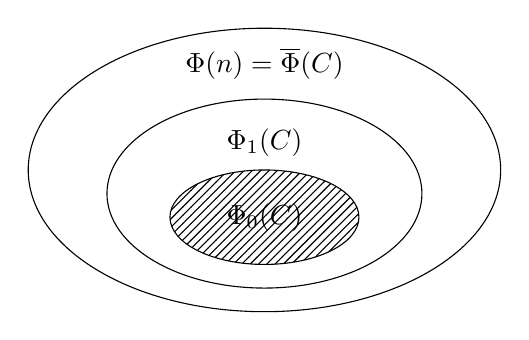
\begin{tikzpicture}[scale=1.0]
        \draw (0, 0) ellipse (3cm and 1.8cm);
        \draw (0, -0.3) ellipse (2cm and 1.2cm);
        \draw[fill opacity=0.4, pattern=north east lines] (0, -0.6) ellipse (1.2cm and 0.6cm);

        \node at (0.0, -0.6) { $\Phi_0(C)$ };
        \node at (0.0, 0.35) { $\Phi_1(C)$ };
        \node at (0, 1.35) { $\Phi(n) = \overline{\Phi}(C)$ };
    \end{tikzpicture}

    \caption{The $n$-implying sets of $\confg$ are increasing in size. If they grow to the set of all ring colorings $\Phi(n)$, the configuration is D-reducible. }
\end{figure}

However, it can occur that $\overline{\Phi}(\confg) \neq \Phi(n)$. This is the case with the ring $R_5$ with a single vertex on the inside, which only supports 3-colorings. To handle (some) of these configurations, a stronger form of D-reducibility was required. This is where we go to C-reducibility.
\section{C-Reducibility}
\label{sec:creduce}

The original proof of the four color theorem used an unavoidable set of C or D reducible configurations. C-reducibility can be thought of as a stronger but more complicated form of D-reducibility. In 2009, John P. Steinberger gave an unavoidable set of D-reducible configurations. With this, C-reducibility is no longer required to prove the four color theorem. However, the concept of C-reducibility is still insightful. Therefore we explain it here.

\subsection{Definitions}

Recall that D-reducibility required that all possible ring colorings $\Phi(n)$ are in the implying set $\overline{\Phi}(C)$. If a configuration is not D-reducible, then there must be ring colorings in $\Phi(n)$ that are not in $\overline{\Phi}(C)$. These colorings can not be converted to coloring of $C$ by flipping Kempe-chains. It is these colorings that we want to avoid with C-reducibility. By replacing $C$ with a reducer $(S,\sigma)$ consisting of a smaller graph $S$ and a ring contraction $\sigma$ we can avoid these colorings. For this to happen, the un-contracted ring colorings of $(S,\sigma)$ denoted by $\Phi(S, \sigma)$ must be in $\overline{\Phi}(C)$.

\begin{figure}[!h]
    \centering
    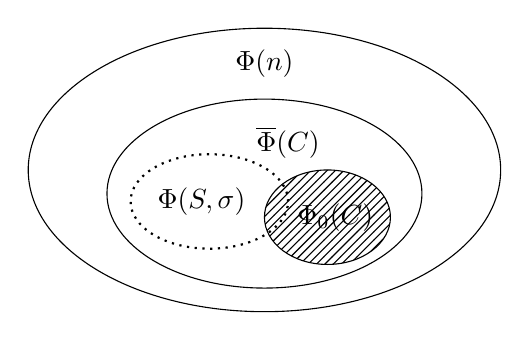
\begin{tikzpicture}[scale=1.0]
        \draw (0, 0) ellipse (3cm and 1.8cm);
        \draw (0, -0.3) ellipse (2cm and 1.2cm);
        \draw[fill opacity=0.4, pattern=north east lines] (0.8, -0.6) ellipse (0.8cm and 0.6cm);
        \draw[dotted, thick] (-0.7, -0.4) ellipse (1.0cm and 0.6cm);

        \node at (0.9, -0.6) { $\Phi_0(C)$ };
        \node at (0.3, 0.35) { $\overline{\Phi}(C)$ };
        \node at (0, 1.35) { $\Phi(n)$ };
        \node at (-0.8, -0.4) { $\Phi(S, \sigma)$ };
    \end{tikzpicture}

    \caption{C-reducibility requires that for some choice of a reducer $(S,\sigma)$, the colorings $\Phi(S, \sigma)$ can be converted to valid ring colorings of $C$ in $\Phi_0(C)$.}
    \label{fig:cred}
\end{figure}

Therefore, C-reducibility can be seen as an extension of D-reducibility with the reducer $(S, \sigma)$ acting as a "filter" of ring colorings. This way we can ignore those ring colorings that are not in $\overline{\Phi}(C)$. As can be seen in Figure \ref{fig:cred}, there are still colorings for the ring that are not in $\overline{\Phi}(C)$. However, we avoid them using the colorings of the reducer $\Phi(S, \sigma)$.

Let us start with the definition of a ring contraction.

\begin{definition}
    A ring contraction $\sigma(v)$ is a map from the vertices of a ring $R$ to the contracted ring $\sigma \circ R$. We require
    
    \begin{itemize}
        \item The contracted ring $\sigma \circ R$ is a valid planar graph.
        \item Neighboring ring vertices $v_i$ and $v_{i+1}$ are not contracted.
    \end{itemize}
\end{definition}

Ring contractions allows the reducer to shrink the number of boundary vertices. This simplifies the coloring problem for the reducer. Without a ring contraction, our reducer would still have the same ring as our configuration $C$, making it equally difficult to work with. Why do we not simply delete vertices from the ring of $C$? The contraction defines a map that allows us to convert boundary colorings of $(S,\sigma)$ to ring colorings of $C$ simply by un-contracting. 

\begin{figure}[!h]
    \centering
    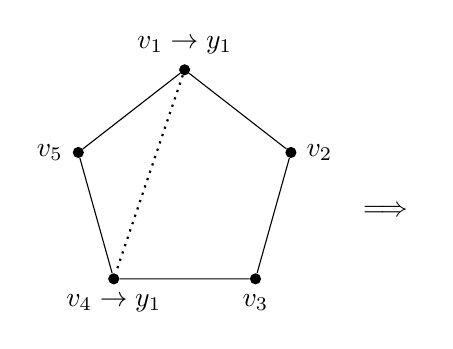
\begin{tikzpicture}[scale=1.5]
        \node[circle, fill, scale=0.015cm, label=above:{$v_1 \rightarrow y_1$}] (l1) at (0, 1) { };
        \node[circle, fill, scale=0.015cm, label=right:{$v_2$}] (l2) at (0.9, 0.30) { };
        \node[circle, fill, scale=0.015cm, label=below:{$v_3$}] (l3) at (0.6, -0.77) {};
        \node[circle, fill, scale=0.015cm, label=below:{$v_4 \rightarrow y_1$}] (l4) at (-0.6, -0.77) {};
        \node[circle, fill, scale=0.015cm, label=left:{$v_5$}] (l5) at (-0.9, 0.30) {};
        \draw (l1) -- (l2) -- (l3) -- (l4) -- (l5) -- (l1);
        \draw[dotted, thick] (l1) -- (l4);
        \node at (1.7, -0.2) { $\implies$ };
    \end{tikzpicture}
    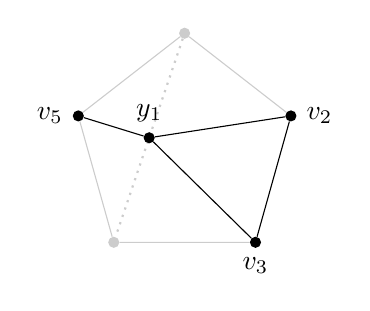
\begin{tikzpicture}[scale=1.5]
        \node[circle, fill, opacity=0.2, scale=0.015cm] (l1) at (0, 1) {};
        \node[circle, fill, opacity=0.2, scale=0.015cm] (l4) at (-0.6, -0.77) {};
        \node[circle, fill, scale=0.015cm, label=above:{$y_1$}] (y1) at (-0.3, 0.115) {};

        \node[circle, fill, scale=0.015cm, label=right:{$v_2$}] (l2) at (0.9, 0.30) { };
        \node[circle, fill, scale=0.015cm, label=below:{$v_3$}] (l3) at (0.6, -0.77) {};
        \node[circle, fill, scale=0.015cm, label=left:{$v_5$}] (l5) at (-0.9, 0.30) {};

        \draw (l5) -- (y1) -- (l2) -- (l3) -- (y1);
        \draw[dotted, thick, opacity=0.2] (l1) -- (l4);
        \draw[opacity=0.2] (l5) -- (l1) -- (l2);
        \draw[opacity=0.2] (l3) -- (l4) -- (l5);
    \end{tikzpicture}
    \caption{A contraction on $R_5$. The two vertices $v_1$ and $v_4$ are mapped to the same vertex $y_1$, and hence get contracted together. }
    \label{fig:contract}
\end{figure}

Figure \ref{fig:contract} shows the contraction process on $R_5$. Intuitively, you should think of a contraction as the merging of pairs of vertices to a single point. However, mathematically, it is easier to work with a mapping function $\sigma$ instead. Suppose we are given a coloring $x(v)$ of a contracted ring $\sigma \circ R$. Then the composition $x \circ \sigma(v)$ is a valid coloring for $R$. This is shown in Figure \ref{fig:contractcolor}

\begin{figure}[!h]
    \centering
    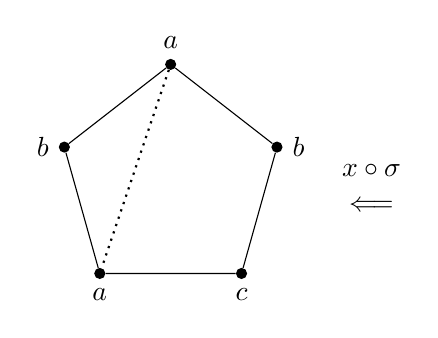
\begin{tikzpicture}[scale=1.5]
        \node[circle, fill, scale=0.015cm, label=above:{$a$}] (l1) at (0, 1) { };
        \node[circle, fill, scale=0.015cm, label=right:{$b$}] (l2) at (0.9, 0.30) { };
        \node[circle, fill, scale=0.015cm, label=below:{$c$}] (l3) at (0.6, -0.77) {};
        \node[circle, fill, scale=0.015cm, label=below:{$a$}] (l4) at (-0.6, -0.77) {};
        \node[circle, fill, scale=0.015cm, label=left:{$b$}] (l5) at (-0.9, 0.30) {};
        \draw (l1) -- (l2) -- (l3) -- (l4) -- (l5) -- (l1);
        \draw[dotted, thick] (l1) -- (l4);
        
        \node at (1.7, 0.1) { $x \circ \sigma$ };
        \node at (1.7, -0.2) { $\Longleftarrow$ };
    \end{tikzpicture}
    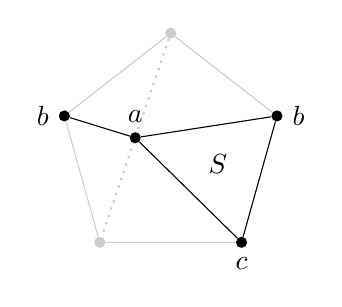
\begin{tikzpicture}[scale=1.5]
        \node[circle, fill, opacity=0.2, scale=0.015cm] (l1) at (0, 1) {};
        \node[circle, fill, opacity=0.2, scale=0.015cm] (l4) at (-0.6, -0.77) {};
        \node[circle, fill, scale=0.015cm, label=above:{$a$}] (y1) at (-0.3, 0.115) {};

        \node[circle, fill, scale=0.015cm, label=right:{$b$}] (l2) at (0.9, 0.30) { };
        \node[circle, fill, scale=0.015cm, label=below:{$c$}] (l3) at (0.6, -0.77) {};
        \node[circle, fill, scale=0.015cm, label=left:{$b$}] (l5) at (-0.9, 0.30) {};

        \draw (l5) -- (y1) -- (l2) -- (l3) -- (y1);
        \draw[dotted, thick, opacity=0.2] (l1) -- (l4);
        \draw[opacity=0.2] (l5) -- (l1) -- (l2);
        \draw[opacity=0.2] (l3) -- (l4) -- (l5);

        \node at (0.4, -0.11) { $S$ };
    \end{tikzpicture}
    \caption{ The coloring $x(v)$ of a contracted ring $\sigma \circ R$ can be converted to a coloring for the original ring $R$ using $x \circ \sigma(v)$. }
    \label{fig:contractcolor}
\end{figure}

By introducing ring contractions, we have already covered the most significant part of a reducer. The last part is the extra graph $S$ that defines the interior of our contracted ring. This extra graph $S$ is similar to the auxiliary graph $A$ that we used during the 1-reducibility proof of $R_5$. The boundary vertices of $S$ must be the same as the contracted ring $\sigma \circ R$. Now we have all the parts needed to define a reducer.

\begin{definition}
    A reducer of a configuration $C$ is a pair $(S, \sigma)$  consisting of a ring contraction $\sigma$ and a graph $S$ on less vertices than $C$ that has a boundary equal to the contracted ring $\sigma \circ R$.
\end{definition}

Of course, every reducer will reduce the size of a configuration $C$. However, for actual reducibility, we can not simply take any reducer. Our reducer $(S, \sigma)$ must satisfy the filtering property mentioned at the beginning of this section. That is, its ring colorings $\Phi(S, \sigma)$ must be contained in $\overline{\Phi}(C)$. Let us define this set.

\begin{definition}
    Let $(S, \sigma)$ be a reducer. The set of un-contracted ring colorings $\Phi(S, \sigma)$ consists of all the colorings $x \circ \sigma$ with $x(v)$ a boundary coloring of $S$.
\end{definition}

Following this definition, C-reducibility is a simple concept.

\begin{definition}
    A configuration $C$ is C-reducible if $\Phi(S,\sigma) \subset \overline{\Phi}(C)$ for some reducer $(S,\sigma)$.
\end{definition}

Now suppose we have a graph $G$ where $C$ is an embedded C-reducible configuration with reducer $(S,\sigma)$. Suppose that two non-neighboring ring vertices of $C$ are connected by an edge in $G$. If we would contract these vertices together, then we would create a loop on the boundary of $S$. We can not color vertices with loops without breaking the rules of a coloring. Therefore, we must take care to avoid such loops.

Since this issue is specific to the way the configuration $C$ is embedded in the graph $G$, we will give a name to the type of embedding that we are after.

\begin{definition}
    A configuration $C$ is $\sigma$-properly embedded in $G$ if two ring vertices of $C$ that are connected by an non-ring edge in $G$ are not contracted by $\sigma(v)$.
\end{definition}

\begin{definition}
    The C-reducible configuration $C$ has a safe reducer  $(S,\sigma)$ if it only occurs $\sigma$-properly embedded in a Birkhoff graph.
\end{definition}

Before we can use C-reducible configurations to reduce counterexamples, we must first prove the existence of a safe reducer. This was a major source of complications in the original proof of the four color theorem by Appel and Haken. This is a strong condition on the structure of a reducer. We will see examples of safe and unsafe reducers in the next section.

\subsection{C-Reducibility of the Birkhoff diamond}
\label{sec:diamond}

Although we have already shown that the Birkhoff diamond is D-reducible, we will use it as a slightly more interesting example of C-reducibility. A reducer for the Birkhoff diamond we have picture below.

\begin{figure}[!h]
    \centering
    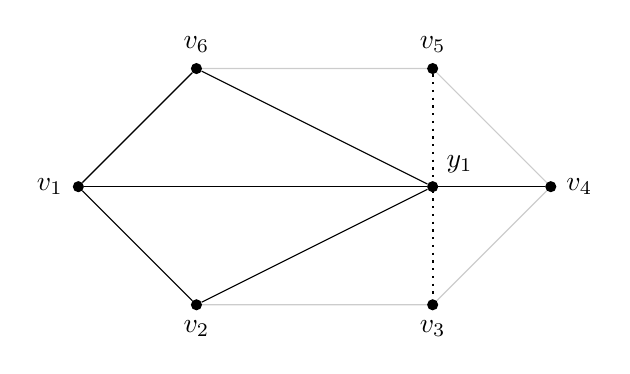
\begin{tikzpicture}[scale=1.5]
        \node[circle, fill, scale=0.015cm, label=left:$v_1$] (l1) at (-2, 0) { };
        \node[circle, fill, scale=0.015cm, label=above:$v_6$] (l2) at (-1, 1) { };
        \node[circle, fill, scale=0.015cm, label=below:$v_2$] (l4) at (-1, -1) {};

        \node[circle, fill, scale=0.015cm,label=right:$v_4$] (r1) at (2, 0) {};
        \node[circle, fill, scale=0.015cm,label=above:$v_5$] (r2) at (1, 1) {};
        \node[circle, fill, scale=0.015cm,label=below:$v_3$] (r4) at (1, -1) {};

        \node[circle, fill, scale=0.015cm,label=above right:$y_1$] (y1) at (1, 0) {};

        \draw[opacity=0.2] (l1) -- (l2) -- (r2) -- (r1) -- (r4) -- (l4) -- (l1);
        \draw[dotted, thick] (r2) -- (r4);
        \draw (l1) -- (l2) -- (y1) -- (l4) -- (l1);
        \draw (l1) -- (y1) -- (r1);
    \end{tikzpicture}
    \caption{A reducer for the Birkhoff diamond (in bold) with a single contraction on $v_4$ and $v_2$, and a single edge added by $S$. }.
    \label{fig:diamondreducer}
\end{figure}

Let us now prove the C-reducibility of the Birkhoff diamond with this reducer. First, we determine the set of colorings that the reducer creates for the original ring $R_6$.

\begin{equation}
    \Phi(S, \sigma) = \left\{ \begin{matrix}
        ababcd, & abcbdc, & abcbcd, \\ abcbac, & abcbad, & \underline{ababac}
    \end{matrix}\right\}
\end{equation}

By looking at Table \
\section{Conclusion}
\section{Conclusions}

\end{document}